% Not All Errors Are Equal: Consequence-Aware Reasoning Compute Allocation
% Target: ICLR 2027 (deadline ~Sept-Oct 2026)

\documentclass{article}
\usepackage{iclr2027_conference,times}

\input{math_commands.tex}

\usepackage[hidelinks,colorlinks=false]{hyperref}
\usepackage{url}
\usepackage{graphicx}
\usepackage{amsmath}
\usepackage{amssymb}
\usepackage{algorithm}
\usepackage{algorithmic}
\usepackage{booktabs}
\title{Not All Errors Are Equal:\\Consequence-Aware Reasoning Compute Allocation}

% The \author macro works with any number of authors. Use \And or \AND
% to break the author list across columns; we go anonymous for submission.
\author{Anonymous authors\\
Paper under double-blind review}

\newcommand{\fix}{\marginpar{FIX}}
\newcommand{\new}{\marginpar{NEW}}

% \iclrfinalcopy % Uncomment for camera-ready (double-blind submission mode when commented)
\begin{document}
\maketitle
\begin{abstract}
Adaptive test-time compute is usually treated as a difficulty-allocation
problem: spend more computation on tasks that are harder or less likely
to be solved. This is natural for average-accuracy benchmarks, where
all errors count equally, but it is incomplete for deployment. A failed
documentation edit and a failed database migration are both one
benchmark error, yet the latter can silently corrupt production data.
Under a fixed compute budget, the relevant question is therefore not
only where the model is likely to fail, but where failure is costly.
We study consequence-aware test-time compute allocation. Each task is
assigned a consequence label measuring the cost of an incorrect answer,
and a deployment-time predictor estimates this consequence from the
issue text and file path before any fix is produced. A scheduler then
routes higher-consequence tasks to stronger compute tiers or more
attempts under the same total budget. The base reasoning model is left
unchanged; the intervention is only a scheduling layer.
Our empirical analysis supports the need for such a layer. On
SWE-bench Lite, consequence is nearly orthogonal to task difficulty, so
high-consequence tasks are not simply the hardest tasks. Five
contemporary thinking models also fail to allocate reasoning compute
reliably by consequence, exhibiting either no consequence signal,
token-budget saturation, or only weak sensitivity. Moreover,
consequence is predictable before solving, whereas the marginal benefit
of extra compute is difficult to predict ex ante.
At a matched compute budget over a 16-system SWE-bench compute tier,
consequence-aware routing shifts success toward the tasks where errors
matter most. The deployment-time scheduler raises high-consequence
success from $19.4\%$ under random routing and $29.0\%$ under
deployment-time predicted difficulty to $51.1\%$, while overall
accuracy is nearly unchanged. This reduces cost-weighted loss by
$21.8\%$ relative to difficulty-aware routing and retains $93.6\%$ of
the oracle-consequence gain. A controlled within-model experiment,
where only best-of-$k$ attempts are reallocated, reproduces the same
ordering. These results suggest that adaptive compute should not be
allocated only by task difficulty, but by the expected cost of being
wrong.
\end{abstract}

\section{Introduction}
\label{sec:intro}

Modern reasoning models can spend different amounts of test-time
computation on different inputs. They may think for more tokens,
sample multiple attempts, call a verifier, or route a task to a
stronger model. This flexibility has motivated a growing line of
adaptive test-time compute methods, where the central question is how
to spend a limited compute budget across a stream of tasks. Most
existing approaches answer this question through difficulty,
confidence, or expected accuracy gain: tasks that appear harder, less
certain, or more likely to benefit from extra computation receive more
compute~\citep{snell2024scaling,damani2024learning,manvi2024adaptive,
qu2026adaptivetesttime}.

This is the right objective for a benchmark that measures average
accuracy. In such a benchmark, every task contributes one unit to the
score, and every failure is interchangeable. But deployment does not
work this way. A coding assistant may fail on a documentation typo,
a parser edge case, a permission check, or a database migration. These
failures may all count as one failed task in a benchmark, yet their
real-world costs differ dramatically. A typo in a log message is
annoying; a migration that silently corrupts production data can be
irreversible. Treating these two errors as equal creates a mismatch
between adaptive-compute objectives and deployment risk.

This paper asks a different question from standard adaptive compute:
under the same total budget, which tasks should the system try hardest
not to get wrong? Our answer is to route computation by
\emph{consequence}, the deployment cost of an incorrect answer. The
goal is not to make every task better. Under a fixed budget, that is
impossible: giving more compute to one task means taking compute away
from another. The goal is instead to reallocate success probability
toward the tasks where failure is most costly. In this view, a good
scheduler may leave average accuracy almost unchanged while greatly
increasing the success rate on high-consequence tasks and reducing
cost-weighted loss.

A natural objection is that difficulty-aware routing might already
capture this effect. Perhaps high-consequence tasks are also the
hardest tasks, or perhaps modern thinking models already spend more
computation when the stakes are high. We find that neither is true.
On SWE-bench Lite, consequence is approximately orthogonal to
difficulty across rule-based, LLM-with-patch, issue-only, and
human-majority labels. High-consequence tasks appear throughout the
difficulty spectrum: some are easy but dangerous, while some very hard
tasks are low consequence. This means that a difficulty-only scheduler
is blind to an important deployment variable. Human-label validation,
rubric ablations, maintainer-revealed severity, cost-mapping
sensitivity, and sub-domain analyses support the same conclusion
(Appendices~\ref{app:iaa}, \ref{app:rubric}, \ref{app:realcost},
\ref{app:costmap}, and~\ref{app:subdomain}).

We also audit whether current reasoning models allocate their own
thinking computation according to consequence. Figure~\ref{fig:motivation}
summarizes the result across five contemporary models. The failure
modes differ by model, but the conclusion is consistent. Qwen3-8B
shows essentially no relationship between thinking length and
consequence ($\rho=0.002$). Qwen3-VL-8B-Thinking and DeepSeek-R1 are
dominated by token-budget saturation, leaving little room for
task-specific allocation. Claude Sonnet~4.5 and o4-mini exhibit weak
positive trends, but high-consequence tasks receive only modestly more
thinking. Thus, existing thinking mechanisms either miss the
consequence signal, saturate their budgets, or adapt too weakly to
serve as deployment-time consequence-aware allocation.

\begin{figure}[t]
\centering
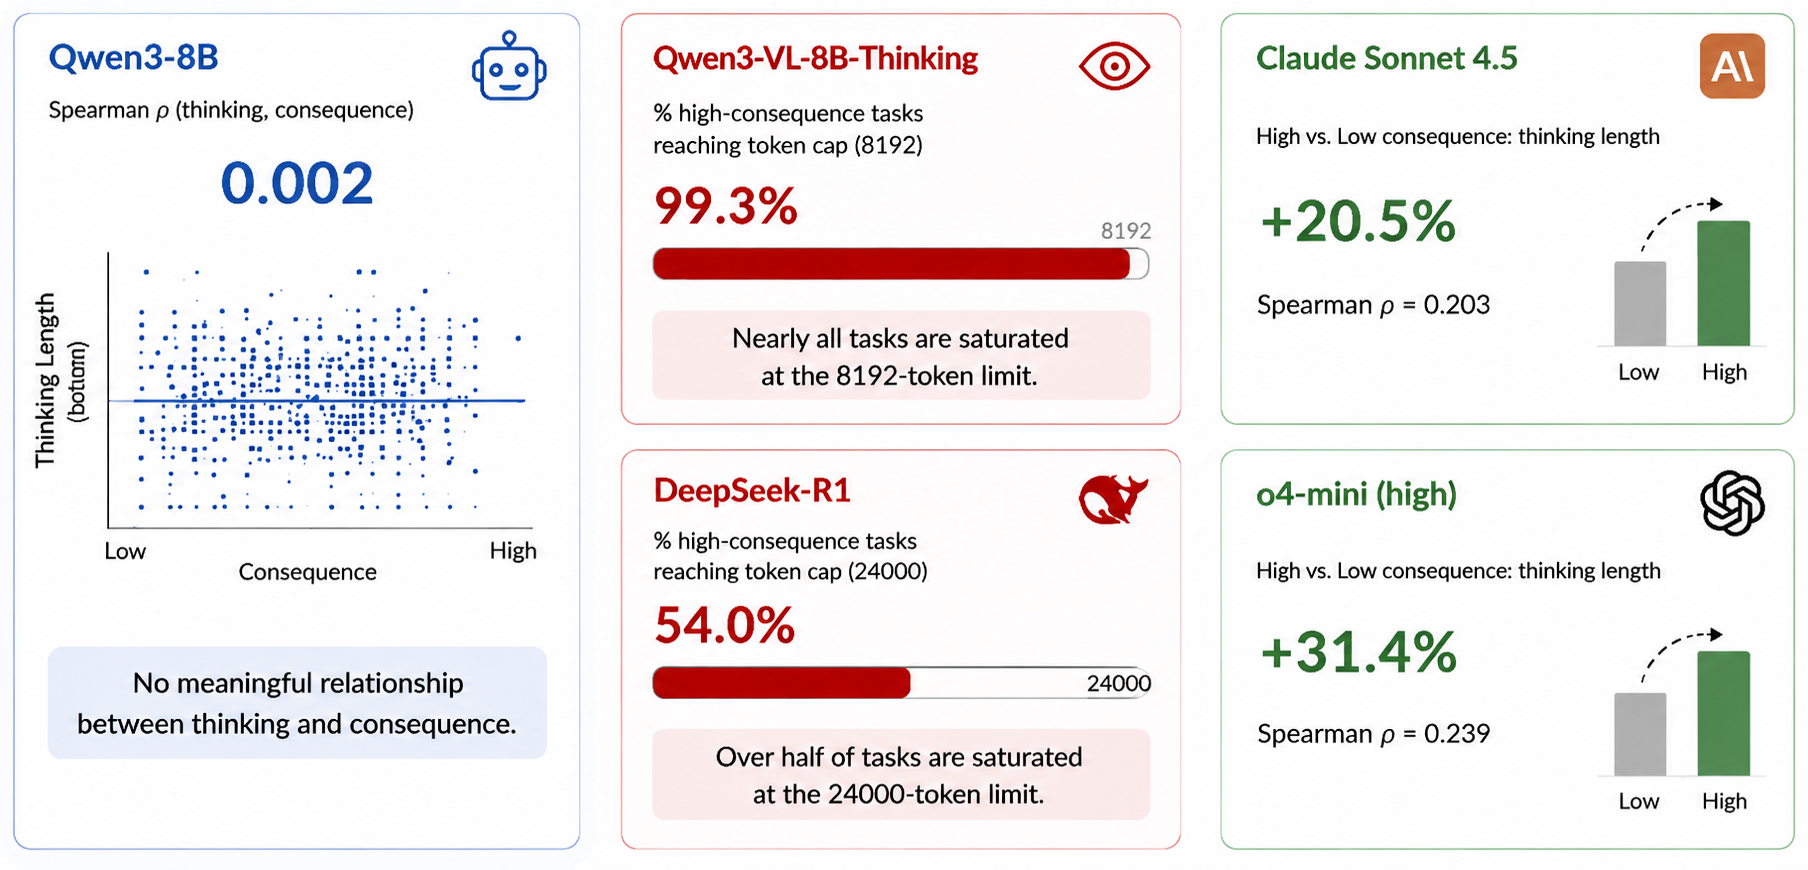
\includegraphics[width=\linewidth]{1.png}
\caption{\textbf{Current reasoning models lack consequence-aware compute allocation.}
We audit five contemporary reasoning models on SWE-bench Lite by measuring
the relationship between thinking computation and task consequence.
Existing models exhibit three failure modes: no consequence sensitivity
(Qwen3-8B, $\rho=0.002$), compute saturation (Qwen3-VL-8B-Thinking:
$99.3\%$ at the 8192-token cap; DeepSeek-R1: $54.0\%$ at the
24000-token cap), or weak adaptation (Claude Sonnet 4.5:
$\rho=0.203$; o4-mini: $\rho=0.239$).}
\label{fig:motivation}
\end{figure}

Motivated by this gap, we introduce consequence-aware test-time
compute allocation. The method is deliberately simple. First, a
deployment-time predictor estimates the consequence of an error from
the issue text and affected file path, without seeing the gold patch,
the final code diff, or any generated fix. Second, a scheduler routes
the highest-consequence tasks to larger compute tiers or more attempts
under the same total budget as a difficulty-based baseline. The base
reasoning model is unchanged; we add no training, no fine-tuning, and
no new reasoning objective. Consequence-awareness enters only through
the scheduling layer.

The key empirical asymmetry is that consequence is available earlier
than marginal compute benefit. Before solving a task, the scheduler can
often infer whether a wrong answer would be costly: issue reports
mention migrations, authentication, deletion, permissions, financial
calculation, or user-visible formatting. By contrast, whether extra
compute will actually change the outcome is much harder to know before
execution. In our experiments, prompted and learned estimators of
marginal gain are near chance before solving, while feedback from a
failed first attempt carries a usable signal for whether retries may
help (Appendix~\ref{app:marginal}). This asymmetry explains why our
deployable scheduler routes by predicted consequence alone, while a
priority-aware analysis variant that additionally uses empirical
marginal gain is treated as an upper-bound-style diagnostic rather
than a deployment-time method.

Our main experiment evaluates this idea on SWE-bench Lite using cached
per-task outcomes from a 16-system compute tier. Each strategy receives
the same premium-compute budget; the only difference is which tasks
are upgraded. The consequence-aware scheduler does not win by improving
all tasks. Instead, it reallocates compute away from low-consequence
tasks and toward high-consequence ones. At the same total budget, the
deployment-time Qwen consequence router raises the success rate on
high-consequence tasks from $19.4\%$ under random routing and
$29.0\%$ under deployment-time predicted difficulty to $51.1\%$,
approaching the all-premium ceiling of $58.5\%$. Overall accuracy
remains essentially unchanged, but cost-weighted loss falls by
$21.8\%$ relative to difficulty-aware routing, retaining $93.6\%$ of
the oracle-consequence gain. A controlled within-model experiment,
where the model and prompt are fixed and only best-of-$k$ attempts are
allocated, reproduces the same ordering; the full protocol, second
judge, dynamic caps, and no-oracle verifier-based sequential policy
are reported in Appendix~\ref{app:within}.

We further analyze why difficulty-aware routing fails in this setting.
The hardest tasks are often not the tasks where extra compute helps
most. On SWE-bench Lite, difficulty is strongly anti-correlated with
the marginal success gain from upgrading to the premium tier
($\rho=-0.78$): many of the hardest tasks remain unsolved even by
premium systems. As a result, difficulty-aware routing can spend its
budget on tasks with little chance of being rescued. Consequence, by
contrast, is not a predictor of where compute helps
($\rho(\mathrm{cons},\Delta\mathrm{success})=+0.09$, n.s.); it
predicts where a successful rescue is valuable. This distinction is
central to the paper: consequence routing is not a better difficulty
estimator. It is a different objective.

The paper makes the following contributions:
\begin{itemize}
\item We formulate test-time compute allocation as a cost-weighted
decision problem, where the objective is consequence-weighted success
under a fixed budget rather than average accuracy alone.

\item We show that consequence is distinct from difficulty and is
predictable before solving. A deployment-time issue-only predictor
recovers high-consequence tasks without access to gold patches or
generated fixes, while existing thinking models do not naturally
allocate computation by consequence.

\item We introduce a deployable consequence-only scheduler that
requires no model retraining or fine-tuning. It ranks tasks by
predicted consequence and routes higher-consequence tasks to larger
compute tiers or more attempts.

\item We demonstrate that consequence-aware routing reallocates
success to the tasks where failure is costly. On SWE-bench Lite,
high-consequence success rises to $51.1\%$ while overall accuracy is
nearly unchanged, reducing cost-weighted loss by $21.8\%$ over
difficulty-aware routing.

\item We validate robustness and boundary conditions through extensive
appendix experiments, including human labels, alternative labelers,
maintainer behavior, cost mappings, predictor calibration, a second
database/ORM software pool, out-of-domain probes, within-model
attempt allocation, live online routing, and context-conditional
consequence labels
(Appendices~\ref{app:iaa}--\ref{app:context}).
\end{itemize}


\section{Related Work}

\textbf{Adaptive test-time compute.}
A growing body of work studies how language models should allocate
test-time computation across inputs. Test-time scaling work analyzes
how performance changes as a function of sampling, verification,
search, or reasoning budget~\citep{snell2024scaling}. Learned
routers and early-exit systems allocate computation by predicted
difficulty, confidence, or expected accuracy gain
\citep{damani2024learning,manvi2024adaptive,qu2026adaptivetesttime}.
A related line routes queries across model cascades, starting from a
cheap model and escalating to a stronger model when confidence is low
or predicted quality is insufficient~\citep{chen2023frugalgpt,
aggarwal2024automix,ong2024routellm,ding2024hybrid}. These methods
differ in mechanism, but they share an accuracy-centered objective:
spend compute where it is expected to improve the probability of a
correct answer. Our work adds a missing term to this objective. In
deployment, the value of a correct answer depends not only on whether
additional compute changes the outcome, but also on how costly the
error would have been.

\textbf{Rational metareasoning.}
The decision-theoretic view of computation as a costly action dates
back to rational metareasoning~\citep{russell1991right,
hay2012selecting}. In that framework, computation should be purchased
only when its expected utility exceeds its cost. Consequence-aware
allocation is a direct instantiation of this idea for modern reasoning
models: the utility of extra computation is the reduction in
consequence-weighted error, not merely the reduction in average error.
Recent work has begun to connect rational metareasoning to large
language models~\citep{yang2024rational}, but most adaptive-compute
systems still operationalize utility as accuracy, confidence, or reward
with uniform error costs. We instead make the task-dependent cost of
being wrong explicit.

\textbf{Cost-sensitive learning and selective prediction.}
Cost-sensitive learning recognizes that different errors can have
different costs~\citep{elkan2001foundations}, while selective
prediction allows a model to abstain when uncertainty is high
\citep{geifman2017selective}. These settings modify the prediction
rule or decide whether to answer. Our setting is different: the model
still answers every task, but the system decides how much computation
to spend before answering. This makes consequence-aware allocation
compatible with existing reasoning models, since the intervention is a
scheduler rather than a retraining objective.

\textbf{Software-engineering benchmarks.}
We use SWE-bench Lite~\citep{jimenez2023swebench} as the primary
testbed because software tasks naturally vary both in difficulty and
in deployment consequence. A formatting bug, a parser bug, a
permission bug, and a database migration error may all appear as
single pass/fail benchmark tasks, while their real-world costs differ
substantially. The benchmark also provides issue reports, file paths,
patches, and public solver outcomes, which allow us to compare
deployment-time consequence prediction with with-patch reference
labels and to evaluate compute allocation under matched budgets. We
validate the construct and routing results with human labels,
maintainer behavior, alternative judges, a second database/ORM
software pool, and out-of-domain probes in the appendix
(Appendices~\ref{app:iaa}--\ref{app:context}).


\section{Consequence as Deployment Error Cost}
\label{sec:cons}

We first define consequence, explain how it is labeled, and show why it
cannot be replaced by task difficulty. This section establishes the
central premise of the paper: high-consequence tasks are not simply the
hardest tasks, so a difficulty-based compute scheduler is not
automatically consequence-aware.

\textbf{Definition.}
We define the consequence of a task as the deployment cost of an
incorrect answer. In this paper we use a coarse ordinal label
$c(x)\in\{0,1,2\}$:
\begin{itemize}\itemsep0pt
  \item \textbf{0 (low).} Cosmetic, formatting, documentation, or
  log-message errors. These may be visible to users but do not corrupt
  downstream systems.
  \item \textbf{1 (medium).} Functional but contained errors, such as
  a wrong return value, a crash on an edge case, or a locally
  recoverable feature failure.
  \item \textbf{2 (high).} Silent data corruption, security or
  permission bypass, irreversible operations such as deletion,
  overwriting, or migration errors, or incorrect results consumed
  downstream without timely visibility.
\end{itemize}
The labels are not intended to be calibrated monetary costs. They are
a minimal ordinal representation of deployment harm, chosen because it
can be applied consistently by both LLM judges and human annotators.
Appendix~\ref{app:costmap} shows that the qualitative allocation
results are stable under alternative monotone mappings and continuous
severity scores.

\textbf{Labeling pipelines.}
We use three labeling modes. First, an LLM-with-patch judge observes
the issue text, the gold patch, and the modified files, and assigns the
reference consequence label used for the main cost-weighted evaluation.
Second, an issue-only predictor observes only deployment-time
information: the GitHub issue text and affected file paths extracted
from the issue report itself, such as stack traces, error logs, or
user-specified file references. It does not receive the gold patch, the
reference modified-file list, or any generated fix. Third, a simple
rule-based labeler provides a lexical baseline. Human annotations,
alternative labelers, and maintainer-revealed severity are used only as
construct-validity checks in the appendix
(Appendices~\ref{app:iaa}, \ref{app:rubric}, and~\ref{app:realcost}).

\textbf{Consequence is not difficulty.}
We measure task difficulty on SWE-bench Lite as
$1-\overline{\mathrm{passrate}}$, where
$\overline{\mathrm{passrate}}$ is the mean success rate of the task
across the 16 public SWE-bench systems used in
\S\ref{sec:exp}. If high-consequence tasks were simply the hardest
tasks, then a difficulty-aware scheduler might already route compute
toward the tasks that matter most. Empirically, this is not the case.
The Spearman correlation between consequence and difficulty is near
zero under both the rule-based labeler
($\rho=+0.047$, $p=0.42$) and the LLM-with-patch reference label
($\rho=-0.096$, $p=0.10$). The same pattern holds for the issue-only
predictor ($\rho=-0.109$, $p=0.06$) and for the human-majority labels
on the annotated subset ($\rho=-0.066$, $p=0.57$;
Appendix~\ref{app:iaa}).

This orthogonality is important for compute allocation. It means that
a scheduler cannot infer deployment risk from difficulty alone. Some
high-consequence tasks are easy but dangerous, such as localized fixes
to deletion, migration, authentication, or data-consistency logic.
Conversely, some very hard tasks have low deployment consequence, such
as obscure formatting or parser edge cases. Routing compute only to
the hardest tasks therefore misses a separate axis of value: which
errors are costly if left uncorrected.

\textbf{Consequence is not merely a confidence signal.}
A second alternative is that consequence may simply reflect model
disagreement or low confidence. We analyze this in
\S\ref{sec:whyfail}. The short version is that consequence is not a
predictor of where extra compute helps; it is a predictor of where a
successful rescue is valuable. Appendix~\ref{app:marginal} further
shows that difficulty and confidence-like signals do not reliably
recover the marginal benefit of extra compute before execution.


\section{Deployment-Time Consequence Prediction}
\label{sec:pred}

A consequence-aware scheduler must make its routing decision before the
model produces a fix. It cannot inspect the gold patch, the final diff,
or the outcome of executing the generated solution. The relevant
question is therefore whether consequence can be estimated from
information available at deployment time.

\textbf{Deployment-time inputs.}
Our predictor receives only the GitHub issue text and file paths that
are explicitly available before solving. In particular, file paths are
included only when they are mentioned in the issue report itself, such
as in stack traces, error logs, or user-specified references. We do not
provide the gold patch, the reference modified-file list, any file path
extracted from the gold diff, or any generated fix. This leakage control
is essential: the predictor is meant to model what a scheduler can know
before deciding how much compute to spend.

\textbf{Predictor.}
We use Qwen2.5-7B-Instruct as the primary issue-only predictor. Given
the deployment-time inputs, it outputs an ordinal consequence label
$\hat{c}(x)\in\{0,1,2\}$ using the same rubric as
\S\ref{sec:cons}. We evaluate it against the LLM-with-patch reference
label, which observes the issue, gold patch, and modified files. This
comparison asks whether the deployment-time signal recovers the
post-hoc consequence assessment closely enough to guide allocation.
As a cross-model robustness check, we also evaluate a Claude
Sonnet~4.5 issue-only predictor against the same with-patch reference.

\textbf{Consequence is predictable before solving.}
On the $300$ SWE-bench Lite tasks, the primary Qwen issue-only
predictor reaches Cohen's $\kappa=0.572$ against the with-patch
reference, indicating moderate agreement on a three-class ordinal
labeling problem. The cross-model Claude predictor reaches
$\kappa=0.379$. These numbers are not perfect, but they show that
consequence is not only a property revealed after seeing the gold
patch: much of it is already present in the issue description and
pre-solution file references.

\textbf{The errors that matter for routing.}
For allocation, the most dangerous predictor error is not an adjacent
label mismatch. It is a severe under-estimation: predicting a
high-consequence task as low consequence, which would route it to the
cheapest compute tier. We therefore focus on the class-$2\to0$ cell.
On SWE-bench Lite, the with-patch reference labels $44$ tasks as
high consequence. The Qwen issue-only predictor identifies $39$ of
them as class~2 and places the remaining $5$ in class~1, yielding
class-2 recall of $88.6\%$ and no high-to-low errors
($2\to0=0/44$). The Claude predictor has lower class-2 recall
($23/44$), but it also makes no high-to-low errors
($2\to0=0/44$). Table~\ref{tab:predictor} summarizes these routing
statistics; full confusion matrices, per-class metrics, threshold
sweeps, and cross-pool calibration are reported in
Appendix~\ref{app:predictor}.

\begin{table}[t]
\centering
\caption{\textbf{Deployment-time consequence prediction on SWE-bench
Lite.} Predictors see only the issue text and pre-solution file paths,
not the gold patch or generated fix. The key routing error is
class-$2\to0$, which would send a high-consequence task to the lowest
compute tier. Both predictors avoid this error on the $44$ true
high-consequence tasks.}
\label{tab:predictor}
\small
\resizebox{\linewidth}{!}{%
\begin{tabular}{lcccc}
\toprule
Predictor & $\kappa$ vs with-patch & Class-2 recall & $2\to0$ & Low--high disagreement \\
\midrule
Qwen2.5-7B-Instruct issue-only
   & $\mathbf{0.572}$ & $\mathbf{88.6\%}$ ($39/44$) & $\mathbf{0/44}$ & $\mathbf{0.0\%}$ ($0/300$) \\
Claude Sonnet~4.5 issue-only
   & $0.379$ & $52.3\%$ ($23/44$) & $\mathbf{0/44}$ & $0.7\%$ ($2/300$) \\
\bottomrule
\end{tabular}%
}
\end{table}

The predictor is deliberately recall-heavy: it over-flags some
medium-consequence tasks as high consequence, but this is the desired
operating point when under-protecting high-consequence tasks is more
costly than wasting some compute on false alarms. Importantly, this
false-alarm cost is already included in the downstream allocation
results of \S\ref{sec:main}; the deployment-time scheduler is evaluated
with the imperfect predictor exactly as used here.

\textbf{Transfer and robustness.}
The same high-to-low safety property holds beyond SWE-bench Lite.
Across the six task pools studied in the paper, the predictor misses
$0$ of $110$ true high-consequence tasks by predicting class~0
(one-sided $95\%$ upper bound $2.7\%$;
Appendix~\ref{app:predictor}). Transfer results on Multi-SWE-bench
mini and on the disjoint database/ORM software pool are reported in
Appendices~\ref{app:crossdataset} and~\ref{app:seconddomain}. These
appendix results are not needed for the main claim, but they support
the use of issue-only consequence as a deployment-time routing signal.



\section{Method: Cost-Weighted Compute Allocation}
\label{sec:method}

The previous sections establish three facts: consequence is a
deployment-relevant error cost distinct from difficulty
(\S\ref{sec:cons}); current thinking models do not reliably allocate
their own computation by consequence (Figure~\ref{fig:motivation} and
Appendix~\ref{app:audit}); and consequence can be estimated before
solving a task (\S\ref{sec:pred}). We now describe how a scheduler uses
this signal under a fixed compute budget.

\textbf{Setup.}
Let $X$ be a stream of tasks and let
$\{T_1,\ldots,T_K\}$ be compute tiers ordered from cheap to expensive.
A tier can correspond to a stronger model, a larger number of attempts,
a verifier-backed procedure, or another deployer-controlled compute
level. Each tier has per-task compute price $c(T_k)$, and the deployer
has a total budget $B$. The scheduler chooses one tier $T(x)$ for each
task.

\textbf{Objective.}
Standard adaptive-compute methods implicitly optimize average accuracy
under a budget. This corresponds to treating all errors as equally
costly. We instead minimize cost-weighted loss:
\begin{equation}
\label{eq:budgetobj}
\min_{T:\,X\to\{T_1,\dots,T_K\}}
\sum_{x\in X}
\mathrm{cost}(x)
\left[
1-p\bigl(\mathrm{correct}\mid x,T(x)\bigr)
\right]
\quad
\mathrm{s.t.}
\quad
\sum_{x\in X} c(T(x)) \le B .
\end{equation}
Here $\mathrm{cost}(x)$ is the consequence weight of task $x$ and
$c(T_k)$ is the compute price of tier $T_k$. When
$\mathrm{cost}(x)\equiv 1$, Eq.~\ref{eq:budgetobj} reduces to the
usual average-accuracy objective. When error costs vary, the scheduler
should spend compute not merely where errors are likely, but where
errors are costly.

Equivalently, since
\[
\sum_x \mathrm{cost}(x)[1-p(x)]
=
\sum_x \mathrm{cost}(x)
-
\sum_x \mathrm{cost}(x)p(x),
\]
minimizing cost-weighted loss is the same as maximizing
consequence-weighted success. This is the key difference from average
accuracy. Under a fixed budget, the scheduler cannot make every task
better. It can only move success probability from some tasks to others.
The purpose of consequence-aware allocation is to move that success
probability toward high-consequence tasks.

\textbf{Exact priority rule.}
Consider the two-tier case with a cheap tier and a premium tier.
Upgrading task $x$ from cheap to premium reduces the objective by
\[
\mathrm{cost}(x)
\left[
p_{\mathrm{premium}}(x)-p_{\mathrm{cheap}}(x)
\right]
=
\mathrm{cost}(x)\Delta(x),
\]
where $\Delta(x)$ is the marginal success gain from extra compute. If
all upgrades have the same compute price, the exact loss-minimizing
allocation upgrades tasks in descending order of
$\mathrm{cost}(x)\Delta(x)$. Thus, the true priority score is not
consequence alone. It is consequence multiplied by marginal compute
benefit.

This decomposition is useful because it separates the two quantities a
deployer would ideally know. The consequence term answers: how costly
is a failure on this task? The marginal-gain term answers: will extra
compute actually change the outcome? The first is often visible before
solving; the second is much harder to estimate before execution.

\textbf{Why the deployable scheduler uses consequence only.}
The exact priority rule requires $\Delta(x)$, but
$\Delta(x)$ is not available before the task is solved. Appendix
\ref{app:marginal} shows that both prompted forecasts and learned
embedding probes fail to predict marginal gain reliably from issue text
alone. In contrast, consequence can be predicted before solving
(\S\ref{sec:pred}). We therefore use a deployment-time approximation:
rank tasks by predicted consequence $\hat{c}(x)$ and allocate the
premium budget to the highest-ranked tasks.

Algorithm~\ref{alg:cons-route} is therefore not the exact optimizer of
Eq.~\ref{eq:budgetobj}. It is the deployable consequence-only
approximation used when marginal-gain estimates are unavailable. In
the fixed-quota experiments of \S\ref{sec:main}, the top-$q\%$ tasks
by $\hat{c}$ receive the premium tier, with $q$ chosen so that total
compute matches the difficulty-aware baseline.

\begin{algorithm}[t]
\caption{Deployable consequence-only compute allocation}
\label{alg:cons-route}
\begin{algorithmic}[1]
\REQUIRE Tasks $X$; deployment-time consequence predictor $\hat{c}$;
tiers $T_1,\ldots,T_K$ with prices $c(T_k)$; total budget $B$.
\STATE Score each task: $s(x) \leftarrow \hat{c}(x)$
\STATE Sort $X$ by $s(\cdot)$ in descending order
\STATE Initialize $T(x) \leftarrow T_1$ for all $x$
\STATE Initialize total cost $C \leftarrow \sum_{x\in X} c(T_1)$
\FOR{$k = K$ down to $2$}
  \FOR{$x$ in sorted order}
    \IF{$T(x) = T_1$ and $C + c(T_k) - c(T_1) \leq B$}
      \STATE $T(x) \leftarrow T_k$
      \STATE $C \leftarrow C + c(T_k) - c(T_1)$
    \ENDIF
  \ENDFOR
\ENDFOR
\RETURN $T$
\end{algorithmic}
\end{algorithm}

This scheduler has three practical properties. First, it does not
modify the reasoning model; all changes happen at the system
scheduling layer. Second, it only requires an ordinal ranking of tasks
by predicted consequence, not calibrated monetary costs. Third, it
fails gracefully: with a perfect consequence predictor it recovers
oracle consequence routing; with an uninformative predictor it reduces
to random routing; and if a difficulty score is substituted for
$\hat{c}$, it becomes a standard difficulty-aware baseline.

\textbf{Analysis variants.}
In the experiments, we also report priority-aware variants that use
empirical $\Delta(x)$ computed from observed cheap- and premium-tier
outcomes. These variants approximate the exact priority rule
$\mathrm{cost}(x)\Delta(x)$ and show the value of knowing where extra
compute changes the outcome. They are analysis variants, not
deployment-time schedulers: the empirical marginal gain is measured
from benchmark outcomes and is unavailable before solving. A split-half
re-estimate of these priority rows is reported in
Appendix~\ref{app:bootstrap} to quantify the optimism introduced by
selecting on empirical gain.


\section{Main Results: Reallocating Success to High-Consequence Tasks}
\label{sec:main}

We now evaluate whether consequence-aware scheduling improves the
allocation of a fixed compute budget. The key question is not whether
the scheduler increases average accuracy on all tasks. Under a fixed
budget, it cannot. The question is whether it moves success toward the
tasks where failure is most costly.

\textbf{Compute-tier setup.}
Our primary experiment uses SWE-bench Lite with cached per-task
outcomes from 16 public SWE-bench systems. These systems span multiple
model generations and agent scaffolds, so the resulting tier system is
best interpreted as a realistic capability ladder rather than a
controlled single-model compute sweep. We sort the 16 systems by total
resolved count and define a cheap tier from the bottom four systems
and a premium tier from the top four systems. For each task $x$,
$p_{\mathrm{cheap}}(x)$ is the fraction of cheap-tier systems that
solve the task, and $p_{\mathrm{premium}}(x)$ is defined analogously
for the premium tier.

All strategies are evaluated under the same matched compute budget:
the top $25\%$ of tasks selected by each strategy are routed to the
premium tier, and the remaining tasks are routed to the cheap tier.
Thus, every strategy spends the same amount of premium compute; only
the identity of the upgraded tasks changes. Appendix~\ref{app:bootstrap}
reports bootstrap confidence intervals, random-allocation variance,
leave-one-class-2-out checks, and split-half estimates for the
priority-aware rows.

\textbf{Strategies.}
We compare random routing, difficulty-aware routing, consequence-aware
routing, and priority-aware analysis variants. Random routes a uniformly
random top-$25\%$ subset of tasks to the premium tier and is averaged
over $1{,}000$ draws. Difficulty-aware routing selects tasks by
difficulty. We include an outcome-derived difficulty baseline
($1-\overline{\mathrm{passrate}}$ across the 16 systems), which is the
strongest difficulty signal available but not deployment-time, and a
deployment-time predicted-difficulty baseline. Consequence-aware
routing selects tasks by predicted consequence $\hat{c}(x)$ from
\S\ref{sec:pred}; the Qwen issue-only predictor is the primary
deployment-time variant, and the Claude issue-only predictor is a
cross-model check. The oracle consequence row uses the with-patch
reference label. Finally, priority-aware rows rank tasks by
$\hat{c}(x)\Delta(x)$ or $c(x)\Delta(x)$, where
$\Delta(x)=p_{\mathrm{premium}}(x)-p_{\mathrm{cheap}}(x)$. Because
$\Delta(x)$ is computed from observed outcomes, these rows are
analysis variants rather than deployment-time methods.

\textbf{Metric.}
We report cost-weighted loss
\[
\mathcal{L}(T)
=
\sum_x c(x)\left[1-p_{T(x)}(x)\right],
\]
where $c(x)$ is the with-patch consequence label and $p_{T(x)}(x)$ is
the success probability of the assigned tier. We also report the
success rate on high-consequence tasks, because this is the most
direct interpretation of the objective: a scheduler that reduces
cost-weighted loss should solve more of the tasks whose failures are
costly. Overall accuracy is included to show whether the effect is a
general accuracy improvement or a reallocation of success.

\begin{table}[t]
\centering
\caption{\textbf{Main routing results on SWE-bench Lite.} All strategies
route the same top-$25\%$ fraction of tasks to the premium tier. The
deployment-time Qwen consequence router raises high-consequence
(class-2) success from $19.4\%$ under random routing and $29.0\%$
under deployment-time predicted difficulty to $51.1\%$, while overall
accuracy is nearly unchanged. The gain is therefore not an average
accuracy gain; it is a reallocation of compute toward tasks where
errors are costly. Priority-aware rows use empirical marginal gain and
are analysis variants rather than deployment-time schedulers.}
\label{tab:main}
\small
\begin{tabular}{lrrrr}
\toprule
Strategy & $\mathcal{L}$ & $\Delta$ vs Diff & class-2 succ. & Acc. \\
\midrule
Difficulty-aware (outcome-derived)                         & $268.25$ & ~~$0\%$ & $6.8\%$ & $0.054$ \\
Difficulty-aware (deployment predicted)                    & $224.00$ & $+16.5\%$ & $29.0\%$ & $0.181$ \\
Random (mean over $1{,}000$ draws)                         & $231.20$ & $+13.8\%$ & $19.4\%$ & $0.180$ \\
\midrule
Consequence-aware (Claude issue-only)                      & $220.50$ & $+17.8\%$ & $36.9\%$ & $0.174$ \\
Consequence-aware (Qwen issue-only; deployment-time)        & $209.75$ & $+21.8\%$ & $\mathbf{51.1\%}$ & $0.184$ \\
Consequence-aware (with-patch oracle)                       & $205.75$ & $+23.3\%$ & $58.5\%$ & $0.187$ \\
\midrule
Priority-aware (Qwen consequence $\times$ marginal gain)    & $\mathbf{186.00}$ & $\mathbf{+30.7\%}$ & $50.6\%$ & $\mathbf{0.274}$ \\
Priority-aware (oracle consequence $\times$ marginal gain)  & $179.75$ & $+33.0\%$ & $55.1\%$ & $0.278$ \\
\bottomrule
\end{tabular}
\end{table}

\textbf{Consequence routing protects the tasks that matter.}
Table~\ref{tab:main} shows the main result. The deployment-time Qwen
consequence router reduces cost-weighted loss by $21.8\%$ relative to
outcome-derived difficulty routing and by $9.3\%$ relative to random
routing. Its oracle counterpart reduces loss by $23.3\%$, so the
deployment-time predictor retains $93.6\%$ of the oracle-consequence
gain measured from the difficulty baseline.

The more important change is visible in the class-2 success column.
Under random routing, high-consequence tasks are solved at $19.4\%$.
Under deployment-time predicted difficulty, they are solved at
$29.0\%$. Under the deployment-time consequence router, they are solved
at $51.1\%$, approaching the all-premium ceiling of $58.5\%$. Overall
accuracy, however, changes little: $0.184$ for the Qwen consequence
router versus $0.180$ for random. This is exactly the intended behavior.
The scheduler is not making the whole benchmark easier; it is moving
compute away from low-consequence tasks and toward high-consequence
tasks. Average accuracy alone would hide this effect.

\textbf{Oracle consequence is close to the deployment-time predictor.}
The gap between the Qwen issue-only router and the with-patch oracle is
small: $209.75$ versus $205.75$ cost-weighted loss. This matters because
the with-patch oracle sees information unavailable at deployment time,
while the issue-only predictor sees only the issue text and pre-solution
file references. The downstream routing result therefore confirms that
the predictor quality in \S\ref{sec:pred} is sufficient for allocation:
it does not need perfect labels, only a useful ranking that avoids
sending high-consequence tasks to the lowest tier. Full tiebreak and
bootstrap analyses are reported in Appendix~\ref{app:bootstrap}.

\textbf{Empirical marginal gain gives an upper-bound-style improvement.}
The priority-aware variants improve further, reaching a $30.7\%$ loss
reduction with predicted consequence and a $33.0\%$ reduction with
oracle consequence. This is expected from Eq.~\ref{eq:budgetobj}: the
exact priority rule ranks by consequence times marginal gain. However,
these rows use empirical $\Delta(x)$ computed from cheap- and
premium-tier outcomes, so they should be read as analysis variants.
They show the value of knowing where extra compute will change the
answer, not a fully deployable solution. Appendix~\ref{app:marginal}
shows that deployment-time predictors of $\Delta(x)$ are unreliable
before execution, and Appendix~\ref{app:bootstrap} reports a split-half
check showing that empirical priority rows are optimistic by roughly
$6$--$7$ percentage points.

\textbf{A controlled within-model compute lever.}
The 16-system experiment is realistic but confounds compute with model
identity and scaffold. We therefore repeat the allocation comparison in
a controlled setting where the model, prompt, and thinking budget are
held fixed, and only the number of best-of-$k$ attempts is allocated.
Using a single Claude Sonnet~4.5 agent, best-of-$k$ provides real
compute headroom: pass rate rises from $\mathrm{pass@}1=0.142$ to
$\mathrm{pass@}8=0.370$. We allocate the same total attempt budget to
each strategy; strategies differ only in which tasks receive more
attempts.

\begin{table}[t]
\centering
\caption{\textbf{Controlled within-model allocation.} A single fixed
Claude Sonnet~4.5 agent is used for all tasks; compute is only the
number of best-of-$k$ attempts. The same strategy ordering holds when
model identity and prompt are fixed, showing that the effect is not an
artifact of routing across heterogeneous model tiers. Full protocol,
second-judge replication, dynamic caps, and no-oracle verifier-based
sequential policies are in Appendix~\ref{app:within}.}
\label{tab:withinmain}
\small
\begin{tabular}{lrrl}
\toprule
Strategy & $\mathcal{L}$ & $\Delta$ vs Diff & bootstrap CI \\
\midrule
Difficulty-aware                         & $102.00$ & ~~$0\%$ baseline & --- \\
Random (mean over $1{,}000$ draws)        & $91.92$  & $+9.9\%$ & --- \\
Consequence-aware (issue-only predictor)  & $83.00$  & $+18.6\%$ & $[+10.5, +30.7]$ \\
Consequence-aware (with-patch oracle)     & $85.00$  & $+16.7\%$ & --- \\
Priority-aware (predictor $\times$ gain)  & $\mathbf{77.00}$ & $\mathbf{+24.5\%}$ & $[+14.6, +35.6]$ \\
\bottomrule
\end{tabular}
\end{table}

Table~\ref{tab:withinmain} reproduces the same qualitative ordering:
difficulty-aware routing is worse than random, consequence-aware
routing improves substantially, and priority-aware routing performs
best. Under the primary judge, the deployment-time consequence
predictor reduces cost-weighted loss by $18.6\%$ relative to
difficulty-aware routing, with a task-level bootstrap interval
$[+10.5,+30.7]$. A second-judge replication preserves the ordering with
smaller but still-positive margins (Appendix~\ref{app:within}). This
controlled experiment addresses the main confound of the 16-system
tier: consequence-aware allocation still helps when the base model is
fixed and the only resource being allocated is additional attempts.

\textbf{Robustness and replication.}
The main result is stable under several checks. Bootstrap resampling,
random-allocation variance, tiebreak analysis, and leave-one-class-2-out
tests are reported in Appendix~\ref{app:bootstrap}. The qualitative
ordering is stable under alternative monotone cost mappings and
continuous severity scores (Appendix~\ref{app:costmap}), and under an
alternative judge family with different severity calibration
(Appendix~\ref{app:judge2}). A second disjoint database/ORM software
pool from SWE-bench Verified reproduces the same strategy ordering with
an independent 20-system tier (Appendix~\ref{app:seconddomain}). These
checks support the main conclusion without changing its interpretation:
the gain comes from reallocating compute toward high-consequence tasks.



\paragraph{Why difficulty routing underperforms.}
Difficulty-aware routing fails in this setting because the hardest
tasks are not the tasks where extra compute has the highest return.
On SWE-bench Lite, outcome-derived difficulty is strongly
anti-correlated with the marginal success gain from the premium tier
($\rho=-0.78$, $p<10^{-60}$): many of the hardest tasks remain
unsolved even by premium systems. Consequence, by contrast, is nearly
uncorrelated with marginal gain ($\rho=+0.09$, n.s.); it does not
predict where compute helps, but where a successful rescue is most
valuable. Appendix~\ref{app:whyfail} gives the full marginal-gain
analysis, including the never-solved decomposition and deployment-time
difficulty estimates. Appendix~\ref{app:marginal} further reports
per-task examples and shows that prompted and learned estimators of
marginal gain are unreliable before execution. The boundary conditions
of this mechanism are tested out of domain in Appendix~\ref{app:ood}.

\section{Conclusion}

Adaptive test-time compute is usually treated as a problem of
difficulty: spend more computation on tasks that are harder, less
certain, or more likely to fail. This paper argues that deployment
requires a second axis. Errors differ in consequence. A system should
therefore decide not only where it is likely to be wrong, but where
being wrong is costly.

We formulated this as a cost-weighted compute-allocation problem and
introduced a deployable consequence-aware scheduler. The scheduler
predicts the consequence of an incorrect answer from deployment-time
inputs, then routes higher-consequence tasks to stronger compute tiers
or more attempts under the same total budget. The base reasoning model
is unchanged; consequence-awareness is added entirely at the scheduling
layer.

The main empirical result is a reallocation of success, not a uniform
accuracy gain. On SWE-bench Lite, the deployment-time scheduler raises
high-consequence success from $19.4\%$ under random routing and
$29.0\%$ under deployment-time predicted difficulty to $51.1\%$,
while overall accuracy remains essentially unchanged. This reduces
cost-weighted loss by $21.8\%$ relative to difficulty-aware routing
and retains most of the oracle-consequence gain. A controlled
within-model experiment, where only best-of-$k$ attempts are
reallocated, reproduces the same ordering.

The results also clarify when consequence-aware routing should and
should not help. Consequence is useful when error costs are
heterogeneous and difficulty is not a reliable proxy for marginal
compute benefit. It should not dominate when costs are uniform, when
premium compute has no headroom, or when harder tasks are exactly the
ones that benefit most from extra compute. The appendix experiments
confirm these boundary conditions across alternative labels, cost
mappings, judges, a second software pool, out-of-domain probes,
sequential policies, online routing, and context-dependent severity.

The broader lesson is that test-time compute allocation should not be
optimized only for average accuracy. In deployment, the value of extra
reasoning depends on what happens if the model is wrong. Consequence is
therefore not a replacement for difficulty or marginal-gain estimation;
it is the missing cost term that determines where successful reasoning
matters most.

\section{Discussion and Limitations}
\label{sec:discussion}

\textbf{Is cost-weighted evaluation circular?}
A natural concern is that consequence-aware routing is evaluated with
the same consequence labels it uses for routing. This concern applies
most directly to the oracle consequence rows, which should indeed be
read as reference points rather than deployable results. The main
deployment-time result is different: the scheduler uses an issue-only
predictor that never sees the gold patch, the generated fix, the final
diff, or benchmark outcomes, and is evaluated against the with-patch
reference labels. Its ability to retain most of the oracle-consequence
gain is therefore an empirical result about pre-solution predictability,
not a tautology. Moreover, the effect is visible in an interpretable
task-level metric: high-consequence success rises sharply while average
accuracy remains nearly unchanged. The result is not merely that a
weighted objective favors a weighted router; it is that a
deployment-time signal shifts solved tasks toward the failures that
would be costly.

\textbf{Consequence labels are coarse but validated.}
Our primary consequence label is produced by an LLM-with-patch judge.
This gives the judge access to the realized fix, but it also raises
construct-validity concerns. We therefore treat the label as a coarse
ordinal deployment-risk weight rather than as ground-truth monetary
cost. Several independent checks support the construct. Human
annotations reproduce the consequence--difficulty orthogonality pattern
and show moderate agreement with the LLM labels
(Appendix~\ref{app:iaa}). Rule-based, issue-only, with-patch, and
human-majority labelings yield the same qualitative allocation
conclusions (Appendix~\ref{app:rubric}). Maintainer-revealed behavior,
including backporting and issue-tracker metadata, aligns with the
consequence classes while remaining distinct from maintainer difficulty
signals (Appendix~\ref{app:realcost}). The routing conclusions are also
stable under alternative monotone cost mappings and continuous severity
scores (Appendix~\ref{app:costmap}) and under an alternative judge
family with different severity calibration (Appendix~\ref{app:judge2}).

\textbf{The method depends on deployment-time consequence prediction.}
The scheduler is only as useful as the pre-solution consequence signal.
In our software pools, the issue-only predictor is deliberately
recall-heavy: it sometimes over-protects medium-consequence tasks, but
it avoids routing true high-consequence tasks to the lowest tier. This
operating point is appropriate when false negatives are more costly
than false positives, and its false-alarm cost is already included in
the allocation numbers. Full calibration details, threshold sweeps, and
cross-pool high-to-low error bounds are reported in
Appendix~\ref{app:predictor}; transfer to Multi-SWE-bench mini and to
the disjoint database/ORM software pool is reported in
Appendices~\ref{app:crossdataset} and~\ref{app:seconddomain}. In
domains where consequence cannot be estimated reliably from
deployment-time inputs, the proposed scheduler should not be used
without a better cost signal.

\textbf{Consequence routing is not universally optimal.}
The paper does not claim that consequence-aware routing always beats
difficulty-aware routing. Eq.~\ref{eq:budgetobj} predicts when each
signal should matter. Consequence routing is useful when error costs
are heterogeneous and difficulty is not a good proxy for marginal
compute benefit. It should lose its advantage when costs are nearly
uniform, when the premium tier has no headroom, or when harder tasks
are precisely the tasks that benefit most from extra compute. The
out-of-domain probes confirm these boundary conditions: the
consequence edge vanishes without meaningful cost heterogeneity, no
routing signal helps without premium headroom, and difficulty routing
wins on competition math where difficulty is positively coupled with
marginal gain (Appendix~\ref{app:ood}). The contribution is therefore
not a universally dominant router, but a decision framework for which
routing signal to use.

\textbf{Marginal-gain estimation remains the hard half.}
The exact priority rule ranks tasks by
$c(x)\Delta(x)$, combining consequence with the marginal success gain
from extra compute. Our priority-aware rows show that this signal would
improve routing if it were known. However, the empirical
$\Delta(x)$ used in those rows is computed from benchmark outcomes and
is not available before solving. Prompted forecasts and learned probes
do not reliably predict this marginal gain from issue text alone
(Appendix~\ref{app:marginal}), and split-half analysis shows that
empirical priority rows are optimistic because they select on noisy
outcome estimates (Appendix~\ref{app:bootstrap}). Execution feedback is
more promising: after a first attempt, verifier scores carry useful
information about whether retries can rescue a task
(Appendix~\ref{app:marginal}). This suggests that ex-ante routing by
consequence and in-flight routing by verifier feedback are
complementary rather than competing approaches.

\textbf{Scope and deployment.}
Our main results use SWE-bench Lite and a second database/ORM software
pool, where consequence heterogeneity is natural and public or cached
solver outcomes allow matched-budget allocation studies. The
within-model experiment removes the model-identity confound by fixing a
single model and allocating only best-of-$k$ attempts
(Appendix~\ref{app:within}). The same appendix also evaluates dynamic
attempt caps and a no-oracle verifier-based sequential policy. A live
online run shows that the routing machinery can operate on streaming
tasks with real-time budget pacing, although that stream lies in a
regime where the framework predicts difficulty rather than consequence
should dominate (Appendix~\ref{app:online}). Finally, consequence is
context-dependent: the same code error can have different severity in a
hobby project, an internal tool, a payment service, or a
safety-critical system. Appendix~\ref{app:context} treats deployment
context as an explicit input and shows that consequence labels and
routing decisions adapt accordingly.


\bibliography{references}
\bibliographystyle{plainnat}

\appendix

\section{Full Audit of Native Thinking Allocation}
\label{app:audit}

This appendix provides the full audit behind Figure~\ref{fig:motivation}.
The goal of the audit is to test whether contemporary reasoning models
already allocate their native thinking computation according to task
consequence. For each model, we measure the relationship between the
amount of thinking computation used on a SWE-bench Lite task and the
LLM-with-patch consequence label defined in \S\ref{sec:cons}.

\begin{table}[h]
\centering
\resizebox{\linewidth}{!}{%
\begin{tabular}{lrrcccl}
\toprule
Model & $n$ & $\mathrm{max\_new}$ &
$\rho(\text{thinking}, \text{cons})$ & $p$ & High vs Low &
Failure mode \\
\midrule
Qwen3-8B (hybrid)              & 300 & 4,096   & +0.002 & n.s.  & ---      & no signal \\
Qwen3-VL-8B-Thinking           & 300 & 8,192   & ---    & ---   & ---      & 99.3\% saturated \\
Claude Sonnet 4.5 (ext. think) & 171 & 16,000  & +0.203 & 0.008 & +20.5\%  & weak but inadequate \\
o4-mini (reasoning API)        & 171 & 12,000  & +0.239 & 0.002 & +31.4\%  & weak but inadequate \\
DeepSeek-R1 (open CoT API)     & 171 & 24,000  & ---    & ---   & ---      & 54\% saturated \\
\bottomrule
\end{tabular}%
}
\caption{\textbf{Native thinking allocation audit on SWE-bench Lite.}
We report sample size, configured token budget, Spearman correlation
between thinking length and consequence, and the observed failure mode.
The audited models exhibit no consequence signal, saturation, or weak
adaptation.}
\label{tab:audit-app}
\end{table}

\paragraph{Qwen3-8B.}
Qwen3-8B is evaluated on all $300$ SWE-bench Lite tasks with
\texttt{max\_new\_tokens}$=4096$. Thinking length varies across tasks,
but its rank correlation with consequence is essentially zero:
$\rho=+0.002$ ($p=0.97$). This is the cleanest ``no signal'' case.

\paragraph{Qwen3-VL-8B-Thinking.}
Qwen3-VL-8B-Thinking reaches the configured token cap on almost every
task: $298/300$ tasks ($99.3\%$) at an $8192$-token cap and
$299/300$ tasks ($99.7\%$) at a $4096$-token cap. With almost all
tasks pinned at the cap, the model has no effective headroom for
task-specific consequence allocation.

\paragraph{Claude Sonnet 4.5.}
Claude Sonnet 4.5 with extended thinking is evaluated on a frozen
$171$-task stratified SWE-bench Lite sample with a $16000$-token
thinking budget. Thinking length has a statistically significant but
small positive correlation with consequence:
$\rho=+0.203$ ($p=0.008$). High-consequence tasks receive $20.5\%$
more thinking than low-consequence tasks on average.

\paragraph{o4-mini.}
OpenAI's o4-mini is evaluated on the same $171$-task sample. Since the
API reports reasoning-token counts, we use those counts as the
per-task compute measure. The correlation is again positive but small:
$\rho=+0.239$ ($p=0.002$), with class-$2$ tasks receiving $31.4\%$
more reasoning tokens than class-$0$ tasks.

\paragraph{DeepSeek-R1.}
DeepSeek-R1 returns an observable reasoning stream. On the same
$171$-task sample, it exhibits a saturation failure mode at frontier
scale: $92\%$ of tasks truncate under an $8192$-token cap, and $54\%$
still truncate under a $24000$-token cap. Among tasks that terminate
naturally, the remaining consequence trend is weak and not
statistically significant.

\paragraph{Interpretation.}
The audit does not show that thinking computation is useless. It shows
that native thinking length is not reliably aligned with the
consequence-weighted objective. This motivates the scheduler-level
intervention of \S\ref{sec:method}: rather than assuming
consequence-awareness emerges from the model's native thinking process,
we add it explicitly at the allocation layer.

\section{Human-Label Robustness Check}
\label{app:iaa}

This appendix validates the consequence construct with human
annotations. The goal is not to replace the full-pool LLM-with-patch
labels, but to test whether the central patterns of the paper survive
under human-majority labels.

\paragraph{Study design.}
We sampled $150$ unique tasks, stratified by the LLM-with-patch
consequence label: $75$ from SWE-bench Lite and $75$ from
Multi-SWE-bench mini. Each annotator received $165$ rows in randomized
order, including $15$ hidden duplicates, five per class, to measure
self-consistency. Three annotators participated: one author, one CS PhD
outside the project, and one non-author CS graduate student. Annotators
did not see the gold patch, file diff, or one another's labels. Each
annotator first completed a $9$-task calibration warm-up with reference
labels.

\paragraph{Self-consistency.}
Cohen's $\kappa$ on the hidden duplicates is $1.000$ for two
annotators and $0.789$ for the third. Raw duplicate agreement is
$100\%$, $100\%$, and $86.7\%$, respectively. The rubric is therefore
internally stable at the annotator level.

\paragraph{Human labels preserve consequence--difficulty orthogonality.}
On the $75$ SWE-bench Lite tasks in the human study, the Spearman
correlation between human-majority consequence and difficulty is
\[
\rho(\mathrm{human\mbox{-}cons},\mathrm{difficulty})=-0.066,
\qquad p=0.57.
\]
This reproduces the main-text conclusion that consequence is not
difficulty. At $n=75$, the study is powered only against correlations
larger than roughly $|\rho|\gtrsim 0.23$, so we interpret this as a
construct-validity check rather than a precise full-pool estimate.

\paragraph{Agreement with LLM labels.}
Table~\ref{tab:human-vs-llm} compares the human-majority labels with
the three labeling pipelines used in the paper.

\begin{table}[h]
\centering
\caption{Cohen's $\kappa$ between human-majority labels and each
labeling pipeline on the $75$ SWE-bench Lite tasks in the human study.}
\label{tab:human-vs-llm}
\small
\begin{tabular}{lc}
\toprule
Pipeline & $\kappa$ vs human majority \\
\midrule
Rule-based labeler & $0.223$ \\
LLM-with-patch judge (Qwen2.5-7B-Instruct) & $0.500$ \\
LLM issue-only predictor (Qwen2.5-7B-Instruct) & $0.517$ \\
\bottomrule
\end{tabular}
\end{table}

The two LLM pipelines show moderate agreement with the human majority,
while the rule-based pipeline is substantially weaker. This supports
using the LLM-with-patch judge as the full-pool primary label, while
treating the human labels as a construct-validity check.

\paragraph{Final human label distribution.}
Of the $150$ tasks, $142$ have a clear majority vote. The remaining
$8$ are three-way splits and are conservatively assigned to the middle
class. The final human-majority distribution is
$\{0{:}45,\ 1{:}67,\ 2{:}38\}$.

\section{Rubric Ablation: All Labeling Pipelines Preserve the Conclusion}
\label{app:rubric}

This appendix checks whether the central findings depend on the
specific LLM-with-patch labeling pipeline used in the main text. We
rerun two analyses under four labelings: rule-based, LLM-with-patch,
LLM issue-only, and human-majority labels.

\paragraph{Orthogonality under all labelings.}
Table~\ref{tab:abl-ortho} reports the Spearman correlation between
consequence and difficulty. All correlations are within $\pm0.11$ of
zero and none is significant at $\alpha=0.05$.

\begin{table}[h]
\centering
\caption{\textbf{Rubric ablation: orthogonality.} Spearman correlation
between consequence and difficulty under four labeling pipelines.}
\label{tab:abl-ortho}
\small
\begin{tabular}{lccc}
\toprule
Labeling pipeline & $n$ & $\rho$ & $p$ \\
\midrule
Rule-based & $300$ & $+0.047$ & $0.42$ \\
LLM-with-patch (paper primary) & $300$ & $-0.096$ & $0.10$ \\
LLM issue-only predictor & $300$ & $-0.109$ & $0.06$ \\
Human majority & $75$ & $-0.066$ & $0.57$ \\
\bottomrule
\end{tabular}
\end{table}

\paragraph{Allocation gain under all labelings.}
For each labeling, we recompute the matched-compute allocation
comparison, using that labeling both as the oracle routing signal and
as the cost weight in the loss. Table~\ref{tab:abl-gain} shows that
priority-aware oracle routing improves over difficulty-aware routing
by $30\%+$ under every labeling.

\begin{table}[h]
\centering
\caption{\textbf{Rubric ablation: allocation gain.} Cost-weighted loss
at the matched top-$25\%$ premium budget, recomputed under each
labeling pipeline.}
\label{tab:abl-gain}
\small
\resizebox{\linewidth}{!}{%
\begin{tabular}{lrrrrrr}
\toprule
Oracle labeling & $n$ & Diff & Random & Cons-oracle & Priority-oracle & $\Delta$ vs Diff \\
\midrule
Rule-based & $300$ & $406.2$ & $352.5$ & $330.8$ & $\mathbf{281.2}$ & $+30.8\%$ \\
LLM-with-patch & $300$ & $268.2$ & $233.8$ & $205.8$ & $\mathbf{179.8}$ & $+33.0\%$ \\
LLM issue-only & $300$ & $307.5$ & $266.2$ & $229.5$ & $\mathbf{201.5}$ & $+34.5\%$ \\
Human majority & $75$ & $75.8$ & $67.5$ & $55.2$ & $\mathbf{48.2}$ & $+36.3\%$ \\
\bottomrule
\end{tabular}%
}
\end{table}

The conclusion is stable: the consequence construct is not an artifact
of one LLM judge or one rubric implementation.

\section{External Validity: Maintainer-Revealed Severity}
\label{app:realcost}

This appendix tests whether the consequence labels align with
maintainer behavior in the real repositories. The premise is that
maintainers reveal severity through costly actions such as backporting
fixes to stable release branches.

\paragraph{Backport mining.}
Each SWE-bench Lite instance encodes its originating pull request. For
$297/300$ tasks with resolvable merge commits, we mined the
corresponding repositories for whether the fix was backported. We also
recorded PR open-to-merge duration, discussion intensity, and security
markers.

\paragraph{Backporting tracks consequence.}
Backport rate increases monotonically with consequence:
\[
8.3\% \ (5/60) \quad \text{for class }0,
\]
\[
20.6\% \ (40/194) \quad \text{for class }1,
\]
\[
41.9\% \ (18/43) \quad \text{for class }2.
\]
The ordered trend is significant ($\rho=+0.232$, $p=0.0001$), and the
class-$2$ vs rest odds ratio is $3.34$ (Fisher $p=0.0009$). Within
the repositories that backport at all, the monotone gradient remains
visible ($19.2\%/36.3\%/47.4\%$) with an ordered trend
$\rho=+0.175$ ($p=0.024$).

\paragraph{Null signals.}
PR open-to-merge duration does not separate consequence classes
(medians $2.0/1.9/1.6$ days; Kruskal--Wallis $p=0.56$). Comment
intensity also does not separate classes (medians $4/5/3$;
$p=0.19$). Security markers are too rare in SWE-bench Lite to be
informative. These nulls are useful: they suggest that backporting
captures severity more directly than general process friction.

\paragraph{Django Trac metadata.}
For the $114$ Django tasks, issue-tracker metadata provides an
LLM-independent anchor. Maintainer-assigned issue type tracks the
consequence label: the fraction labeled as genuine ``Bug'' rises from
$26.7\%$ at class~0 to $69.7\%$ at class~1 and $78.8\%$ at class~2
(ordered trend $\rho=+0.282$, $p=0.002$). The ``easy pickings''
difficulty flag is approximately orthogonal to consequence
($\rho=-0.12$, n.s.). Thus, maintainer behavior supports the paper's
central separation between consequence and difficulty.

\section{Statistical Robustness of Allocation Results}
\label{app:bootstrap}

This appendix quantifies the stability of Table~\ref{tab:main}. We
report tiebreak variance, split-half priority estimates, task-level
bootstrap intervals, random-allocation variance, and a
leave-one-class-2-out analysis.

\paragraph{Tiebreak variance.}
Ordinal consequence scores create ties. Re-drawing the tiebreak vector
$1{,}000$ times gives predictor loss $210.2\pm1.8$ with $95\%$
interval $[206.8,213.5]$ and oracle-consequence loss $206.4\pm2.0$.
The headline retention of oracle-consequence gain has mean $93.9\%$
and $95\%$ interval $[85.9\%,102.5\%]$.

\paragraph{Split-half priority estimates.}
Priority-aware rows select tasks using empirical marginal gain
estimated from the same tier outcomes used for evaluation. This is
optimistic because of selection on noise. Splitting each tier in half,
selecting on one half and evaluating on the other over $200$ random
splits, gives $+27.2\%\pm1.6$ for oracle priority, compared with
$+33.8\%$ when selecting and evaluating on the same half. The priority
rows should therefore be read as optimistic by roughly $6$--$7$ points.

\paragraph{Task-level bootstrap.}
We resample the $300$ SWE-bench Lite tasks with replacement $5{,}000$
times. Table~\ref{tab:bootstrap} reports percentile intervals.

\begin{table}[h]
\centering
\caption{\textbf{Task-level bootstrap} over $5{,}000$ resamples at the
top-$25\%$ matched-compute operating point.}
\label{tab:bootstrap}
\small
\resizebox{\linewidth}{!}{%
\begin{tabular}{lrrrr}
\toprule
Strategy & $\mathcal{L}$ & $95\%$ CI & $\Delta$ vs Diff & $95\%$ CI \\
\midrule
Difficulty-aware & $268.25$ & $[249.2,286.8]$ & baseline & --- \\
Random & $231.20$ & $[214.8,251.2]$ & $+13.8\%$ & $[+9.9,+16.2]\%$ \\
Consequence-aware (Claude issue-only) & $220.50$ & $[201.2,239.8]$ & $+17.8\%$ & $[+14.1,+21.5]\%$ \\
Consequence-aware (Qwen issue-only) & $209.75$ & $[190.8,230.0]$ & $+21.8\%$ & $[+17.6,+25.5]\%$ \\
Consequence-aware (with-patch oracle) & $205.75$ & $[187.0,223.8]$ & $+23.3\%$ & $[+19.2,+27.4]\%$ \\
Priority-aware (Qwen + gain) & $186.00$ & $[169.5,203.0]$ & $+30.7\%$ & $[+27.7,+33.4]\%$ \\
Priority-aware (oracle + gain) & $179.75$ & $[163.0,197.5]$ & $+33.0\%$ & $[+30.3,+35.4]\%$ \\
\bottomrule
\end{tabular}%
}
\end{table}

\paragraph{Random allocation variance.}
At the fixed task set, $1{,}000$ independent random top-$25\%$
allocations have mean loss $231.20$, standard deviation $3.70$, and
$95\%$ interval $[224.0,238.2]$. All $1{,}000$ random allocations
outperform outcome-derived difficulty routing.

\paragraph{Leave-one-class-2-out.}
Removing each of the $44$ high-consequence tasks in turn, the Qwen
issue-only consequence router remains within $[+21.5,+22.3]\%$
reduction over difficulty-aware routing and wins in all $44$ runs. The
priority-aware row remains within $[+30.3,+30.9]\%$ and also wins in
all $44$ runs.

\section{Cost-Mapping and Continuous-Severity Sensitivity}
\label{app:costmap}

The main text maps consequence classes $\{0,1,2\}$ directly to scalar
weights. This appendix tests whether the results depend on that
particular mapping.

\paragraph{Monotone mappings.}
Table~\ref{tab:costmap} recomputes the matched-compute comparison
under five monotone cost mappings. The ordering
Consequence-aware $>$ Random $>$ Difficulty-aware and
Priority-aware $>$ Consequence-aware is preserved under every mapping.

\begin{table}[h]
\centering
\caption{\textbf{Cost-mapping sensitivity.} Cost-weighted loss and
relative reduction over difficulty-aware routing under alternative
mappings of consequence classes to scalar weights.}
\label{tab:costmap}
\small
\resizebox{\linewidth}{!}{%
\begin{tabular}{lrrrrrr}
\toprule
Mapping & Diff & Random & Cons-Qwen & Cons-oracle & Pri-Qwen & Pri-oracle \\
\midrule
$\{0,1,2\}$  & $268.2$  & $231.2$ & $209.8$ ($+21.8\%$) & $205.8$ ($+23.3\%$) & $186.0$ ($+30.7\%$) & $179.8$ ($+33.0\%$) \\
$\{1,2,3\}$  & $552.0$  & $482.0$ & $454.5$ ($+17.7\%$) & $449.8$ ($+18.5\%$) & $398.2$ ($+27.9\%$) & $393.2$ ($+28.8\%$) \\
$\{1,2,5\}$  & $634.0$  & $551.5$ & $497.5$ ($+21.5\%$) & $486.2$ ($+23.3\%$) & $448.2$ ($+29.3\%$) & $435.2$ ($+31.3\%$) \\
$\{1,3,10\}$ & $1025.2$ & $888.8$ & $771.8$ ($+24.7\%$) & $746.8$ ($+27.2\%$) & $697.0$ ($+32.0\%$) & $672.8$ ($+34.4\%$) \\
$\{0,1,5\}$  & $391.2$  & $337.2$ & $274.2$ ($+29.9\%$) & $260.5$ ($+33.4\%$) & $249.5$ ($+36.2\%$) & $236.5$ ($+39.6\%$) \\
\bottomrule
\end{tabular}%
}
\end{table}

\paragraph{Continuous severity weights.}
We also elicit continuous $0$--$100$ severity scores from two judge
families, \texttt{deepseek-chat} and GPT-4o, on both SWE pools. The
continuous scores correlate with the ordinal labels
($\rho=0.38$--$0.49$ across judge-pool combinations) and with each
other (cross-judge Spearman $0.50$ on Lite and $0.40$ on Verified).
Re-running allocation with continuous scores as loss weights preserves
the ordering in all four combinations.

\begin{table}[h]
\centering
\caption{\textbf{Allocation under continuous $0$--$100$ severity
weights.} The deployment route remains the ordinal issue-only
predictor; loss weights and oracle routing use continuous severity.}
\label{tab:contcost}
\small
\resizebox{\linewidth}{!}{%
\begin{tabular}{llrrrrr}
\toprule
Pool & Weights & Random & Cons-pred & Cons-oracle$_{\mathrm{cont}}$ & Pri-pred & Pri-oracle$_{\mathrm{cont}}$ \\
\midrule
Lite & deepseek-chat & $+13.1\%$ & $+16.7\%$ & $+20.6\%$ & $+25.3\%$ & $+31.5\%$ \\
Lite & GPT-4o        & $+13.9\%$ & $+17.8\%$ & $+20.8\%$ & $+27.6\%$ & $+30.7\%$ \\
Verified & deepseek-chat & $+12.5\%$ & $+14.2\%$ & $+18.7\%$ & $+26.4\%$ & $+30.9\%$ \\
Verified & GPT-4o        & $+13.7\%$ & $+13.8\%$ & $+22.6\%$ & $+25.2\%$ & $+30.1\%$ \\
\bottomrule
\end{tabular}%
}
\end{table}

\section{Predictor Calibration Details}
\label{app:predictor}

This appendix expands \S\ref{sec:pred} with full confusion matrices,
per-class metrics, operating thresholds, and cross-pool safety
statistics.

\paragraph{Qwen issue-only predictor.}
Against the Qwen2.5-7B-Instruct with-patch reference on $300$
SWE-bench Lite tasks, the issue-only predictor reaches
$\kappa=0.572$. The confusion matrix is:
\[
\begin{array}{c|ccc|c}
& \hat{c}=0 & \hat{c}=1 & \hat{c}=2 & \text{total} \\\hline
c=0 & 47 & 13 & 0 & 60 \\
c=1 & 11 & 140 & 45 & 196 \\
c=2 & 0 & 5 & 39 & 44 \\\hline
\text{total} & 58 & 158 & 84 & 300
\end{array}
\]
Per-class precision/recall/F1 are: class~0
$(0.81/0.78/0.80)$, class~1 $(0.89/0.71/0.79)$, and class~2
$(0.46/0.89/0.61)$. The class-$2\to0$ cell is $0/44$.

\paragraph{Claude issue-only predictor.}
The cross-model Claude Sonnet~4.5 predictor reaches $\kappa=0.379$.
The confusion matrix is:
\[
\begin{array}{c|ccc|c}
& \hat{c}=0 & \hat{c}=1 & \hat{c}=2 & \text{total} \\\hline
c=0 & 33 & 25 & 2 & 60 \\
c=1 & 25 & 148 & 23 & 196 \\
c=2 & 0 & 21 & 23 & 44 \\\hline
\text{total} & 58 & 194 & 48 & 300
\end{array}
\]
Per-class precision/recall/F1 are: class~0
$(0.57/0.55/0.56)$, class~1 $(0.76/0.76/0.76)$, and class~2
$(0.48/0.52/0.50)$. The class-$2\to0$ cell is again $0/44$.

\paragraph{Operating thresholds across pools.}
The ordinal predictor can be thresholded either at $\hat{c}=2$ or
$\hat{c}\ge1$ for detecting class-$2$ tasks.

\begin{center}
\small
\begin{tabular}{lccc}
\toprule
Pool & true $2$s & recall / precision ($\hat{c}=2$) & recall / precision ($\hat{c}\ge1$) \\
\midrule
Lite      & $44$ & $0.89$ / $0.46$ & $1.00$ / $0.18$ \\
MSWE mini & $3$  & $1.00$ / $0.16$ & $1.00$ / $0.01$ \\
Verified  & $47$ & $0.96$ / $0.62$ & $1.00$ / $0.37$ \\
BIRD      & $3$  & $1.00$ / $0.20$ & $1.00$ / $0.03$ \\
FinQA     & $10$ & $0.60$ / $1.00$ & $1.00$ / $0.09$ \\
MATH      & $3$  & $0.00$ / ---    & $1.00$ / $0.04$ \\
\bottomrule
\end{tabular}
\end{center}

Across all six pools, the predictor misses $0/110$ true
high-consequence tasks by predicting class~0. The one-sided
$95\%$ Clopper--Pearson upper bound on the high-to-low miss rate is
$2.7\%$.

\section{Per-Task Marginal Utility and Marginal-Gain Prediction}
\label{app:marginal}

This appendix supports the method and discussion around the exact
priority rule
\[
\mathrm{priority}(x)=c(x)\Delta\mathrm{success}(x).
\]
It documents per-task marginal utility, deployment-time attempts to
predict marginal gain, and the role of execution feedback.

\paragraph{Per-task examples.}
Table~\ref{tab:marg} contrasts tasks selected by priority with tasks
selected by raw difficulty.

\begin{table}[h]
\centering
\caption{Per-task marginal utility excerpt. Priority-ranked tasks have
moderate difficulty and high marginal gain; difficulty-ranked tasks sit
in the unsalvageable tail.}
\label{tab:marg}
\small
\begin{tabular}{lcccc}
\toprule
Selection & cons & difficulty & $\Delta$success & priority \\
\midrule
\multicolumn{5}{l}{\textit{Top-8 by priority}} \\
top-1 & $2$ & $0.50$ & $1.00$ & $2.00$ \\
top-2 & $2$ & $0.50$ & $1.00$ & $2.00$ \\
top-3 & $2$ & $0.56$ & $0.75$ & $1.50$ \\
top-4 & $2$ & $0.56$ & $0.75$ & $1.50$ \\
top-5 & $2$ & $0.62$ & $0.75$ & $1.50$ \\
top-6 & $2$ & $0.62$ & $0.75$ & $1.50$ \\
top-7 & $1$ & $0.31$ & $1.00$ & $1.00$ \\
top-8 & $1$ & $0.31$ & $1.00$ & $1.00$ \\
\midrule
\multicolumn{5}{l}{\textit{Top-4 by difficulty}} \\
top-1 & $1$ & $1.00$ & $0.00$ & $0.00$ \\
top-2 & $1$ & $1.00$ & $0.00$ & $0.00$ \\
top-3 & $2$ & $1.00$ & $0.00$ & $0.00$ \\
top-4 & $0$ & $1.00$ & $0.00$ & $0.00$ \\
\bottomrule
\end{tabular}
\end{table}

\paragraph{Prompted marginal-gain prediction.}
We prompted \texttt{deepseek-chat} and GPT-4o to forecast the success
probability of a basic agent and a frontier agent from issue text and
file path alone. The absolute success levels are moderately
predictable, with $\rho$ up to $+0.39$, but the difference
$\hat{\Delta}$ is not: correlations with true
$\Delta\mathrm{success}$ lie between $-0.07$ and $+0.05$ across
family-pool combinations.

\paragraph{Learned marginal-gain probe.}
A ridge regression probe on issue-text embeddings
(\texttt{text-embedding-3-small}, 10-fold task-level cross-validation)
also fails to predict marginal gain reliably:
$\rho(\hat{\Delta},\Delta)=+0.11$ on Lite ($p=0.06$) and
$+0.13$ on Verified (n.s.). AUC for detecting $\Delta>0$ is $0.49$
on Lite and $0.34$ on Verified, and cross-pool transfer is near zero.

\paragraph{Execution feedback carries signal.}
After a first failed attempt, a gold-free verifier score becomes
informative. Among tasks whose first attempt fails, the verifier score
predicts whether attempts $2$--$8$ rescue the task with
$\rho=+0.23$ ($p=0.016$, AUC $0.65$) under the Claude judge and
$\rho=+0.21$ ($p=0.027$, AUC $0.65$) under the DeepSeek judge. This
supports the distinction used in the main text: marginal gain is hard
to estimate before execution, but in-flight feedback can support
sequential allocation.

\section{Why Difficulty-Aware Allocation Fails}
\label{app:whyfail}

This appendix provides the full marginal-gain analysis summarized in
\S\ref{sec:main}.

\paragraph{Marginal gain.}
Let
\[
\Delta\mathrm{success}(x)
=
p_{\mathrm{premium}}(x)-p_{\mathrm{cheap}}(x).
\]
This quantity measures where premium compute changes the outcome.

\begin{figure}[h]
\centering
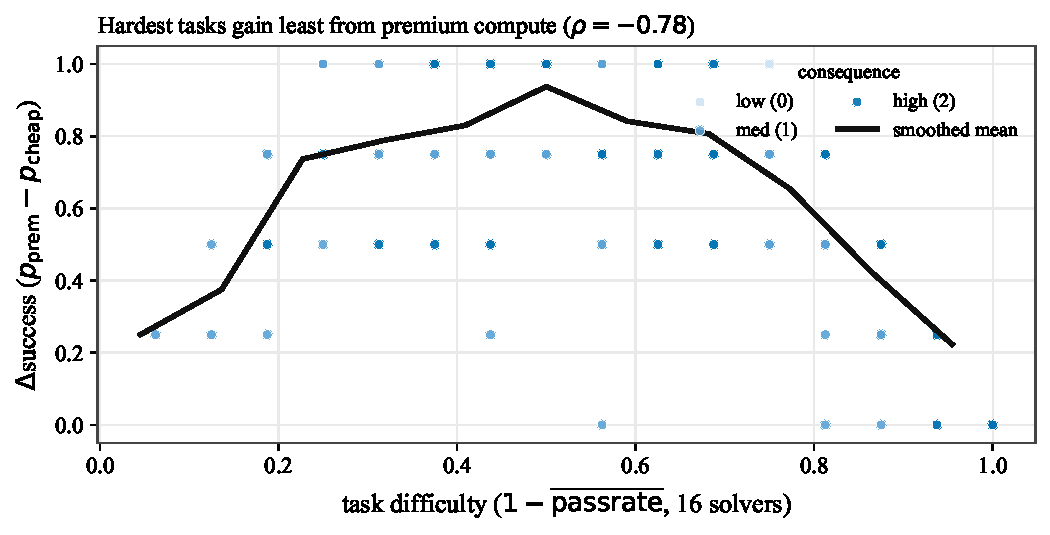
\includegraphics[width=\linewidth]{fig_marginal.pdf}
\caption{\textbf{Difficulty and marginal gain on SWE-bench Lite.}
Marginal gain collapses on the hardest tasks, producing
$\rho(\mathrm{difficulty},\Delta\mathrm{success})=-0.78$
($p<10^{-60}$).}
\label{fig:marginal-app}
\end{figure}

\paragraph{Difficulty anti-selects marginal gain.}
On SWE-bench Lite,
\[
\rho(\mathrm{difficulty},\Delta\mathrm{success})=-0.78,
\qquad p<10^{-60}.
\]
Many of the hardest tasks remain unsolved even at the premium tier, so
upgrading them consumes compute without changing outcomes.

\paragraph{Not only a never-solved artifact.}
There are $76/300$ tasks solved by no system. Removing them, the
correlation remains strongly negative:
\[
\rho=-0.489,\qquad p<10^{-14}.
\]
Thus, the pattern is not purely caused by the never-solved floor.

\paragraph{Deployment-time difficulty estimates.}
Issue-only solvability forecasts from two model families produce
difficulty estimates whose correlation with marginal gain is weak and
not significant: $-0.087$ and $+0.058$ on Lite, and $-0.051$ and
$-0.144$ on Verified. Routing by these deployment-time difficulty
estimates lands near random and below consequence routing.

\paragraph{Consequence and marginal gain.}
Consequence is nearly uncorrelated with marginal gain:
\[
\rho(\mathrm{consequence},\Delta\mathrm{success})=+0.09
\quad \text{(n.s.)}.
\]
Consequence therefore does not predict where compute helps. It predicts
where help is valuable if it occurs.

\paragraph{Boundary conditions.}
The same decomposition predicts when consequence routing should fail:
when costs are homogeneous, when premium compute has no headroom, or
when difficulty is positively coupled with marginal gain. Appendix
\ref{app:ood} tests these cases out of domain.

\section{Robustness Across SWE-bench Sub-Domains}
\label{app:subdomain}

This appendix checks whether the main findings are driven by a
particular sub-domain of SWE-bench Lite. We define heuristic
sub-domains using lexical filters and rerun orthogonality, predictor
agreement, and allocation analyses inside each group.

\begin{table}[h]
\centering
\caption{\textbf{Robustness across SWE-bench Lite sub-domains.}
$\rho$ is the correlation between consequence and difficulty,
$\kappa$ is predictor agreement with the with-patch reference,
$2\to0$ is the high-to-low error count, and $\Delta$ vs Diff is the
priority-aware oracle gain over difficulty-aware routing.}
\label{tab:subdomain}
\small
\begin{tabular}{lrrrrr}
\toprule
Sub-domain & $n$ & $\rho(\mathrm{cons},\mathrm{diff})$ & $\kappa$ & $2\to0$ & $\Delta$ vs Diff \\
\midrule
Numeric / scientific computing    & $36$  & $-0.13$ & $0.52$ & $0$ & $+30.2\%$ \\
Parsers / CLI / tokens            & $35$  & $-0.10$ & $0.69$ & $0$ & $+33.1\%$ \\
Rendering / UI / formatting       & $61$  & $+0.13$ & $0.61$ & $0$ & $+30.6\%$ \\
Imports / modules / configuration & $141$ & $-0.08$ & $0.53$ & $0$ & $+30.7\%$ \\
\bottomrule
\end{tabular}
\end{table}

The same pattern holds across sub-domains: consequence remains weakly
related to difficulty, the predictor avoids high-to-low errors, and
priority-aware routing improves over difficulty-aware routing.

\section{Cross-Dataset Transfer: Multi-SWE-bench mini}
\label{app:crossdataset}

This appendix evaluates transfer of the consequence construct and
issue-only predictor to Multi-SWE-bench mini.

\paragraph{Pool structure.}
The pool is structurally low-consequence. The with-patch judge assigns
only $3/400$ tasks ($0.75\%$) to class~2, compared with $44/300$
($14.7\%$) on SWE-bench Lite. Most tasks are class~1.

\paragraph{Predictor transfer.}
On $399$ doubly labeled tasks, the Qwen issue-only predictor reaches
Cohen's $\kappa=0.382$ with raw agreement $72.2\%$:
\[
\begin{array}{c|ccc|c}
& \hat{c}=0 & \hat{c}=1 & \hat{c}=2 & \text{total} \\\hline
c=0 & 67 & 39 & 1 & 107 \\
c=1 & 56 & 218 & 15 & 289 \\
c=2 & 0 & 0 & 3 & 3 \\\hline
\text{total} & 123 & 257 & 19 & 399
\end{array}
\]
All three class-$2$ tasks are recovered, and the high-to-low cell is
again empty.

\paragraph{Why no allocation study.}
We do not run a matched-compute allocation study on Multi-SWE-bench
mini because no public per-task multi-model outcome table is available
for constructing cheap and premium tiers, and because the pool contains
only three high-consequence tasks. Appendix~\ref{app:seconddomain}
therefore provides the second full software allocation study on a
class-$2$-rich database/ORM pool.

\section{A Second Software Pool: Database/ORM Tasks from SWE-bench Verified}
\label{app:seconddomain}

This appendix repeats the full allocation comparison on a disjoint
pool of $140$ database/ORM tasks from SWE-bench Verified.

\paragraph{Pool construction.}
We select \texttt{django/django} tasks whose issue text or touched
files match database/ORM signals: migrations, schema, SQL, querysets,
transactions, integrity constraints, and related terms. We exclude all
instances overlapping the main SWE-bench Lite pool. Compute tiers are
built from $20$ public SWE-bench Verified leaderboard submissions,
using the bottom four systems as cheap tier and the top four as
premium tier.

\paragraph{Consequence distribution.}
The with-patch judge assigns $47/140$ tasks ($33.6\%$) to class~2,
making this a consequence-rich software pool. The full distribution is
$\{0{:}8,\ 1{:}85,\ 2{:}47\}$.

\paragraph{Predictor transfer.}
The Qwen issue-only predictor reaches $\kappa=0.582$ with raw
agreement $75.7\%$:
\[
\begin{array}{c|ccc|c}
& \hat{c}=0 & \hat{c}=1 & \hat{c}=2 & \text{total} \\\hline
c=0 & 8 & 0 & 0 & 8 \\
c=1 & 4 & 53 & 28 & 85 \\
c=2 & 0 & 2 & 45 & 47 \\\hline
\text{total} & 12 & 55 & 73 & 140
\end{array}
\]
Class-$2$ recall is $45/47$ ($95.7\%$), and the class-$2\to0$ cell is
again empty.

\paragraph{Allocation replication.}
Table~\ref{tab:seconddomain} repeats the matched-compute comparison.

\begin{table}[h]
\centering
\caption{\textbf{Second-pool allocation} on $140$ database/ORM tasks
from SWE-bench Verified with an independent $20$-system tier.}
\label{tab:seconddomain}
\small
\begin{tabular}{lrr}
\toprule
Strategy & $\mathcal{L}$ & $\Delta$ vs Diff \\
\midrule
Difficulty-aware (oracle difficulty) & $154.75$ & $0\%$ \\
Random (mean over $1{,}000$ draws) & $135.61$ & $+12.4\%$ \\
Consequence-aware (Qwen issue-only) & $131.75$ & $+14.9\%$ \\
Consequence-aware (with-patch oracle) & $121.00$ & $+21.8\%$ \\
Priority-aware (pred $\times$ empirical gain) & $111.25$ & $+28.1\%$ \\
Priority-aware (oracle $\times$ empirical gain) & $\mathbf{106.00}$ & $\mathbf{+31.5\%}$ \\
\bottomrule
\end{tabular}
\end{table}

The strategy ordering exactly replicates the main pool:
difficulty-aware is worst, random is better, consequence-aware improves
further, and priority-aware is best.

\section{Judge Robustness for Consequence Labels}
\label{app:judge2}

This appendix tests whether the results depend on the Qwen2.5-7B
with-patch judge. We relabel both SWE pools with
\texttt{deepseek-chat} using the same with-patch rubric prompt.

\paragraph{Judges calibrate severity differently.}
On SWE-bench Lite, Qwen and DeepSeek agree at $\kappa=0.182$ with raw
agreement $48.0\%$. DeepSeek is much more severe, assigning $54.7\%$
of Lite tasks to class~2 versus $14.7\%$ for Qwen. On the Verified
database/ORM pool, agreement is $\kappa=0.140$.

\paragraph{Ordering is mostly preserved.}
On Lite under DeepSeek weights, difficulty-aware remains worst
($435.25$), random improves ($378.31$, $+13.1\%$), consequence-aware
improves further ($362.75$, $+16.7\%$), and priority-aware is best
(up to $305.75$, $+29.8\%$). On Verified, difficulty-aware is also
worst and priority-aware best, while consequence-only matches random
because DeepSeek assigns class~2 to most of the pool, flattening cost
heterogeneity.

\paragraph{Interpretation.}
Judge swaps reveal a threshold-calibration issue, not a collapse of
the construct. When a judge flattens the cost distribution by marking
most tasks high consequence, consequence-only routing has little room
to outperform random. This is consistent with the objective: the value
of consequence routing depends on perceived cost heterogeneity.

\section{Out-of-Domain Probes: BIRD, FinQA, and MATH}
\label{app:ood}

This appendix tests the framework outside SWE-style software repair.
The goal is not to show that consequence always wins, but to test the
boundary conditions predicted by the objective.

\paragraph{BIRD text-to-SQL.}
We sample $150$ questions from BIRD dev, stratified over business
databases and official difficulty labels. The cheap tier is GPT-4o-mini
and the premium tier is o4-mini, with three samples per task per tier.
Execution accuracy rises from $44.0\%$ to $53.3\%$, giving modest
headroom.

Under the primary Qwen weights, costs are nearly homogeneous:
only $3/150$ tasks are class~2. Consequence routing therefore collapses
toward random, as predicted. Under a GPT-4o judge that assigns higher
stakes to medical, toxicological, and financial queries, consequence
becomes more useful.

\begin{table}[h]
\centering
\caption{\textbf{BIRD text-to-SQL allocation} under two judge weightings.}
\label{tab:ood-bird}
\small
\begin{tabular}{lrrrr}
\toprule
& \multicolumn{2}{c}{Qwen weights} & \multicolumn{2}{c}{GPT-4o weights} \\
Strategy & $\mathcal{L}$ & $\Delta$ & $\mathcal{L}$ & $\Delta$ \\
\midrule
Difficulty-aware & $66.67$ & $0\%$ & $75.00$ & $0\%$ \\
Random & $68.27$ & $-2.4\%$ & $75.80$ & $-1.1\%$ \\
Consequence-aware (question-only pred) & $67.33$ & $-1.0\%$ & $72.67$ & $+3.1\%$ \\
Consequence-aware (with-gold oracle) & $65.67$ & $+1.5\%$ & $66.67$ & $+11.1\%$ \\
Priority-aware (pred $\times$ gain) & $58.00$ & $+13.0\%$ & $62.00$ & $+17.3\%$ \\
Priority-aware (oracle $\times$ gain) & $\mathbf{56.33}$ & $\mathbf{+15.5\%}$ & $\mathbf{62.00}$ & $\mathbf{+17.3\%}$ \\
\bottomrule
\end{tabular}
\end{table}

\paragraph{FinQA.}
On $150$ FinQA questions, premium reasoning compute provides almost no
headroom. o4-mini scores below the cheap tier ($64.2\%$ vs $66.2\%$),
and GPT-4o adds only $+1.1$ points. With no meaningful premium
headroom, all routing signals land near random. This is exactly the
objective's prediction: if upgrading rarely helps, choosing where to
upgrade cannot matter.

\paragraph{MATH.}
On $150$ MATH problems, premium compute has large headroom
($65.3\%\to82.3\%$), and difficulty is positively coupled with
marginal gain:
\[
\rho(\mathrm{level},\Delta\mathrm{success})=+0.257,
\qquad p=0.002.
\]
Here difficulty routing wins, because harder math problems are exactly
where the premium reasoning tier helps. This is the opposite regime
from SWE-bench.

\paragraph{Boundary-condition summary.}
\begin{center}
\small
\begin{tabular}{lcccl}
\toprule
Pool & top-$25\%$ weight share & $\rho(\mathrm{diff},\Delta)$ & headroom & best deployable signal \\
\midrule
SWE Lite & $0.42$ & $-0.78$ & yes & consequence \\
SWE Verified DB/ORM & $0.39$ & $-0.38$ & yes & consequence \\
BIRD & $0.35$ & $+0.06$ & modest & none / near random \\
FinQA & $0.36$ & $+0.01$ & none & none \\
MATH & $0.50$ & $+0.26$ & large & difficulty \\
\bottomrule
\end{tabular}
\end{center}

\paragraph{Declared dollar stakes.}
We additionally run a controlled stakes sweep on FinQA and MATH. Stakes
tiers are assigned orthogonally to difficulty, and the cost spread
between low and high stakes is swept from $1\times$ to $10^6\times$.

\begin{table}[h]
\centering
\caption{Declared-stakes sweep: margin of consequence-aware over
difficulty-aware routing as dollar-cost spread increases.}
\label{tab:stakescross}
\small
\begin{tabular}{lrrrrrrr}
\toprule
Spread $S$ & $1$ & $3$ & $10$ & $30$ & $100$ & $10^3$ & $10^6$ \\
\midrule
MATH margin & $-28.3\%$ & $-18.4\%$ & $-6.5\%$ & $+3.2\%$ & $+11.5\%$ & $+20.2\%$ & $+24.9\%$ \\
MATH cons wins & $0\%$ & $0\%$ & $26\%$ & $62\%$ & $76\%$ & $84\%$ & $84\%$ \\
FinQA margin & $+2.9\%$ & $+3.6\%$ & $+4.4\%$ & $+5.1\%$ & $+5.7\%$ & $+6.3\%$ & $+6.6\%$ \\
FinQA cons wins & $84\%$ & $78\%$ & $76\%$ & $76\%$ & $76\%$ & $76\%$ & $76\%$ \\
\bottomrule
\end{tabular}
\end{table}

The sweep quantifies when cost heterogeneity can override difficulty:
on MATH, consequence routing flips from losing to winning between
$10\times$ and $30\times$ cost spread.

\section{Within-Model Allocation: Attempts as the Compute Lever}
\label{app:within}

This appendix provides the full protocol for the controlled
within-model experiment summarized in \S\ref{sec:main}.

\paragraph{Thinking-token budget as a weak lever.}
We first test thinking-token budgets on two families. For Claude
Sonnet~4.5, sweeping budgets
$\{1024,2048,4096,8192,16000\}$ on an $80$-task stratified sample
produces no consistent success improvement; pass rates are
$0.100/0.064/0.100/0.150/0.100$. For DeepSeek-R1, increasing hard caps
$\{4096,8192,16000,24000\}$ raises success only from $1/80$ to
$7/80$, with zero class-$2$ successes at every cap. Budget-level
allocation is therefore degenerate on these tasks.

\paragraph{Attempts as a real compute lever.}
We fix a Claude Sonnet~4.5 agent with the same prompt and thinking
budget and vary only the number of attempts. On the scaled sample,
best-of-$k$ pass rate rises from $\mathrm{pass@}1=0.142$ to
$\mathrm{pass@}8=0.370$, giving real compute headroom.

\paragraph{Original 48-task experiment.}
In the original sample, $48$ tasks receive all eight attempts. The
matched budget is $216$ attempts: $24$ tasks at best-of-$8$ and
$24$ tasks at a single attempt. Results are:

\begin{table}[h]
\centering
\caption{\textbf{Original within-model allocation} on $48$ tasks.}
\label{tab:within}
\small
\begin{tabular}{lrr}
\toprule
Strategy & $\mathcal{L}$ & $\Delta$ vs Diff \\
\midrule
Difficulty-aware & $36.0$ & $0\%$ \\
Random & $30.0$ & $+16.7\%$ \\
Consequence-aware (issue-only predictor) & $29.0$ & $+19.4\%$ \\
Consequence-aware (oracle) & $27.0$ & $+25.0\%$ \\
Priority-aware (pred $\times$ gain) & $27.0$ & $+25.0\%$ \\
Priority-aware (oracle) & $\mathbf{26.0}$ & $\mathbf{+27.8\%}$ \\
\bottomrule
\end{tabular}
\end{table}

Bootstrap intervals are wide but positive: $[+6.5,+44.1]\%$ for
consequence-aware and $[+11.6,+47.2]\%$ for priority-aware.

\paragraph{Scaled 127-task experiment.}
We extend to $127$ tasks with all eight attempts under the Claude
judge. Difficulty-aware loss is $102.00$, random $91.92$,
consequence-aware issue-only $83.00$ ($+18.6\%$), oracle consequence
$85.00$ ($+16.7\%$), and priority-aware predictor $77.00$
($+24.5\%$). The task-level bootstrap interval is
$[+10.5,+30.7]\%$ for consequence-aware and $[+14.6,+35.6]\%$ for
priority-aware. A stricter DeepSeek judge on $126$ tasks preserves the
ordering with smaller margins: consequence-predictor $+8.7\%$ and
priority $+13.5\%$.

\paragraph{Dynamic caps with oracle verifier.}
We also evaluate sequential policies offline. Attempts are issued one
at a time and stop at first success. Consequence-gated caps dominate:
under the Claude judge, a deployment-time profile
$k_{\max}=2/8/8$ by predicted class matches uniform best-of-$8$ loss
while consuming $20\%$ fewer attempts; the oracle-gated version saves
$28\%$. Difficulty-gated caps do not match uniform-$8$ loss at lower
budget.

\paragraph{Gold-free verifier.}
Replacing the oracle verifier with a gold-free \texttt{deepseek-chat}
verifier, consequence-gated caps match uniform best-of-$8$ loss at
$31$--$42\%$ less realized compute across judges and acceptance
thresholds. Difficulty-gating adds little beyond a uniform lower cap.
This is the fully deployable sequential stack: issue-only consequence
predictor, gold-free verifier, and consequence-gated attempt caps.

\paragraph{Judge agreement.}
On the original attempt set, Claude and DeepSeek judges agree on
$91.3\%$ of attempts with Cohen's $\kappa=0.630$. Recomputing the
allocation comparison under DeepSeek verdicts preserves the same
ordering.

\section{A Live Online Deployment Run}
\label{app:online}

This appendix evaluates whether the routing machinery can run as a
live streaming system rather than an offline replay.

\paragraph{Setup.}
A stream of $300$ tasks, $150$ FinQA plus $150$ MATH, arrives one at a
time. Tasks carry deployment-declared stakes mapped to
\$10K/\$1M/\$10M. Four policies process the same stream under a
real-time premium budget: random, difficulty, consequence, and a
verifier-gated sequential policy. The run uses live calls to
\texttt{gpt-4o-mini}, \texttt{gpt-4o}, and \texttt{o4-mini}. Routing
components never see gold answers; grading is post-hoc.

\paragraph{Results.}
\begin{table}[h]
\centering
\caption{\textbf{Live online run} on a $300$-task FinQA+MATH stream.}
\label{tab:online}
\small
\begin{tabular}{lrrrl}
\toprule
Policy & DWL & loss red.\ vs random & premium & accuracy \\
\midrule
\textsc{random} & $24{,}426$ & $0\%$ & $23.0\%$ & $70.0\%$ \\
\textsc{diff} & $\mathbf{16{,}432}$ & $\mathbf{+32.7\%}$ & $25.3\%$ & $70.7\%$ \\
\textsc{cons} & $19{,}831$ & $+18.8\%$ & $19.3\%$ & $68.7\%$ \\
\textsc{seq} & $21{,}627$ & $+11.5\%$ & $\mathbf{5.0\%}$ & $70.0\%$ \\
\bottomrule
\end{tabular}
\end{table}

The stream lies in a regime where the framework predicts difficulty,
not consequence, should dominate because MATH has positive
difficulty--gain coupling. The live run confirms this. The
verifier-gated sequential policy uses only $5.0\%$ premium calls while
matching random accuracy, showing that the machinery can operate online
with real-time budget pacing.

\paragraph{Scope.}
This is not a live consequence-wins demonstration. It shows that the
routing system works online and respects the predicted boundary
conditions. A production online run in the SWE-style regime remains
future work.

\section{Context-Conditional Consequence}
\label{app:context}

Consequence depends on deployment context. The same error can be low
severity in a hobby project and high severity in a payment or
safety-critical system. This appendix treats context as an explicit
input:
\[
c(x) \rightarrow c(x,\mathrm{context}).
\]

\paragraph{Setup.}
For $100$ stratified SWE-bench Lite tasks, we elicit continuous
severity scores under four declared deployment contexts: a personal
hobby project, an internal business tool with human review, a
payment-processing service, and a safety-critical industrial control
system. We use two judge families, \texttt{deepseek-chat} and GPT-4o,
in both with-patch and issue-only modes, producing $1600$ labels.

\paragraph{Severity shifts monotonically with context.}
Mean severity rises monotonically along the stakes ladder. For
DeepSeek with-patch labels, the means are
$22.9 \to 26.2 \to 50.6 \to 64.7$. For GPT-4o, they are
$27.4 \to 28.4 \to 34.2 \to 42.5$. The shift is often monotone within
individual tasks as well: non-decreasing severity appears for
$71\%$ of tasks under DeepSeek and $90\%$ under GPT-4o in judge mode.

\paragraph{Routing adapts to context.}
Using each context's with-patch severity as the weight and the same
context's issue-only severity as the routing signal, consequence
routing beats random in all eight context-by-judge cells
($+6.1\%$ to $+10.9\%$) and difficulty routing in all eight
($+17.5\%$ to $+23.5\%$). The selected premium sets differ across
contexts: overlap between the top-$25\%$ sets under hobby and
safety-critical contexts is only $36\%$ under DeepSeek and $52\%$
under GPT-4o.

\paragraph{Interpretation.}
Context-dependence is not a threat to consequence-aware allocation; it
is an input to it. The scheduler can condition on deployment context
when the deployer provides it.



\end{document}